\chapter{Introduction}

Since creating, refining and managing grids in general is a very
complex topic which has severe effects on computational efficiency and
for which no generic and efficient approach exists, our simulation
framework is build on top of DUNE, the \textbf{D}istributed and \textbf{U}nified
\textbf{N}umerics \textbf{E}nvironment~\cite{DUNE-HP}. DUNE provides a generic interface to many
grid management libraries such as UG~\cite{UG-HP}, ALBERTA~\cite{ALBERTA-HP},
ALU-Grid~\cite{ALUGRID-HP} and a few more. DUNE extensively uses templates in
order to achieve maximum efficiency to access the actual grid
libraries\footnote{In fact, the performance penalty resulting from the
  use of DUNE's grid interface is usually negligible~\cite{BURRI2006}.}.
\begin{figure}[hbt]
  \centering 
  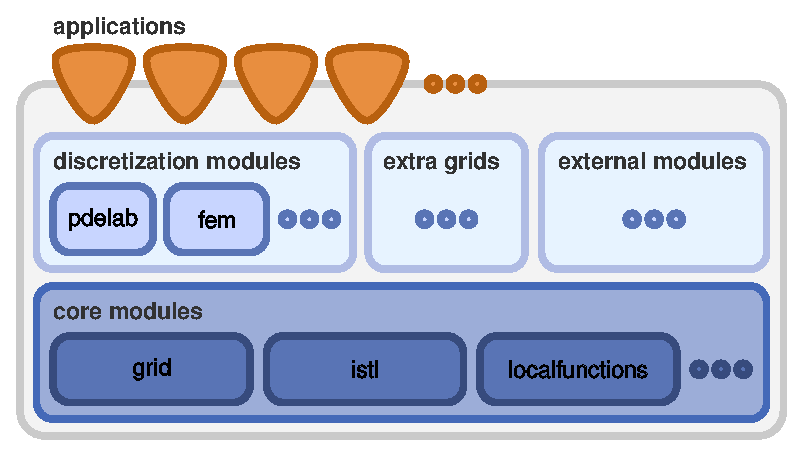
\includegraphics[width=.5\linewidth, keepaspectratio]{EPS/dunedesign}
  \caption{
    \label{fig:dune-design}
    A high-level overview on DUNE's design as available on the project's
    web site~\cite{DUNE-HP}.
  }
\end{figure}

DUNE's grid interface is independent of the spatial dimension of the
underlying grid. For this purpose, it uses the concept of
co-dimensional entities. Roughly speaking, an entity of co-dimension
$0$ constitutes a cell, co-dimension $1$ entities are faces between
cells, co-dimension $1$ are edges, and so on until co-dimension $n$
which are the cell's vertices.  The DUNE grid interface generally
assumes, that all entities are convex polytopes, which means that it
must be possible to express each entity as the convex hull of a set of
vertices. For efficiency, all entities are further expressed in terms
of so-called reference elements which are transformed to the actual
spatial incarnation within the grid by a so-called geometry
function\footnote{The same approach is also used by \texttt{dune-disc} for
  finite element shape functions.}. Here, a reference element for an
entity can be thought of as a prototype for the actual grid
entity. For example, if we used at a grid that used hexahedrons as cells,
the reference element for each cell would be the unit cube $[0, 1]^3$
and the geometry function would scale and translate the cube so that
it matches the grid's cell. For a more thorough description of DUNE's
grid definition, see~\cite{BASTIAN2008}.

In addition to the grid interface, DUNE also provides quite a few additional
modules, of which the \texttt{dune-disc} and \texttt{dune-istl} modules are the most
relevant in the context of this handbook.  \texttt{dune-disc} provides a toolbox for
discretization and includes a set of generic finite element shape
functions, matrix assemblers for translating local stiffness matrices
into global linear systems of equations and much more. \texttt{dune-istl} is the
\textbf{I}terative \textbf{S}olver \textbf{T}emplate \textbf{L}ibrary
and provides generic, highly optimized linear algebra routines for solving
the generated systems. 

DuMu$^\text{x}$ comes in form of an additional module \texttt{dune-mux}. 
It inherits functionality from all available DUNE modules. 
Its main intention is to provide a framework for easy and efficient 
implementation of models from porous media flow problems, 
ranging from problem formulation, the selection of 
spatial and temporal discretization schemes, as well as nonlinear solvers,  
up to general concepts for model coupling.  
Moreover, DuMu$^\text{x}$ includes ready to use numerical models and example applications. 

